\section{Planificación inicial del trabajo}

El desarrollo del presente Trabajo Fin de Grado se ha planteado inicialmente según una planificación estructurada a tres niveles: temporal, de recursos y económico. Esta planificación se organizó siguiendo un modelo en cascada, en el que cada fase se apoya en los resultados de la anterior.

\subsection{Planificación temporal}

El desarrollo del proyecto se ha llevado a cabo a lo largo de varios meses, iniciándose en septiembre y finalizando en junio, siguiendo una estructura secuencial por fases:

\subsubsection{Fase 1: Recolección y análisis de requisitos} (septiembre – octubre)
Esta primera fase se centra en la recolección y el análisis de los requisitos del sistema, estableciendo una base para el posterior desarrollo. 
\begin{itemize}
    \item \textbf{Creación de un documento de requisitos:} Se elaborará un documento detallado que incluya tanto los requisitos funcionales como los no funcionales del sistema. Este se usará como referencia para el resto de etapas del proyecto. 
    \item \textbf{Redacción de historias de usuario:} Para capturar los requisitos desde la perspectiva del usuario final, se redactarán historias de usuario detalladas que describan las funcionalidades deseadas. Estas ayudarán a mantener el enfoque en el objetivo del usuario durante todo el desarrollo.
    \item \textbf{Diagramas de casos de uso:} Se crearán diagramas de casos de uso para representar gráficamente las interacciones entre los usuarios y el sistema, asegurando una comprensión clara de los flujos de trabajo y ayudando a la identificación de posibles brechas en los requisitos.
\end{itemize}

\subsubsection{Fase 2: Diseño} (noviembre – diciembre)
En la segunda etapa se desarrolla el diseño detallado del sistema, asegurando el cumplimiento de los requisitos especificados durante la etapa anterior.
\begin{itemize}
    \item \textbf{Definición de la arquitectura del sistema:} Se decidirá la estructura general del sistema, incluyendo la elección de tecnologías, plataformas y patrones de diseño. Esto garantiza que el sistema soporte los requisitos funcionales y no funcionales establecidos.
    \item \textbf{Creación de diagramas de clases:} Se desarrollarán diagramas de clases detallados que muestren la estructura del sistema, incluyendo las relaciones entre las distintas clases y sus atributos y métodos. Estos proporcionarán una vista clara de cómo los diferentes componentes del sistema interactúan entre sí.
    \item \textbf{Desarrollo de wireframes:} Se diseñarán wireframes que representen esquemáticamente la interfaz de usuario. Los wireframes realizados se podrán utilizar como guía visual inicial, mostrando la disposición de los elementos en la pantalla.
    \item \textbf{Diagramas de flujo:} Se crearán diagramas de flujo para representar la interacción del usuario con el sistema, desde la navegación entre pantallas hasta la ejecución de las diferentes funciones. 
    \item \textbf{Prototipo funcional:} Se desarrollará un prototipo interactivo que simule la apariencia y el comportamiento del producto final, permitiendo tanto la realización de pruebas de usabilidad como la validación del diseño antes del desarrollo. Proporciona la oportunidad de realizar ajustes antes de realizar otras etapas más costosas.
\end{itemize}

\subsubsection{Fase 3: Implementación y experimentación} (enero – abril)
Esta fase se centra en la implementación del sistema, transformando el diseño detallado en las etapas anteriores en un código funcional.
\begin{itemize}
    \item \textbf{Escritura del código:} Se procederá a la codificación de los diferentes componentes del sistema siguiendo las especificaciones y el diseño definidos. Se aplicarán los estándares establecidos para garantizar la calidad y la consistencia del código.
    \item \textbf{Integración de componentes:} Se integrarán los módulos y componentes del sistema, asegurando que funcionen de manera cohesiva y que se comuniquen correctamente entre sí. Será testeada mediante tests de integración para verificar su funcionamiento.
    \item \textbf{Revisión del código:} Se realizará una revisión exhaustiva del código desarrollado utilizando, si es necesario, herramientas automatizadas para asegurar su calidad, mantenibilidad a largo plazo y el cumplimiento de los requisitos y estándares.
\end{itemize}

\subsubsection{Fase 4: Integración, pruebas y validación} (mayo)
En esta última fase del proyecto se verifican y validan los componentes para asegurar que se cumplen los requisitos establecidos.
\begin{itemize}
    \item \textbf{Desarrollo de un plan de pruebas:} Se elaborará un plan detallado que especificará los tipos de pruebas a realizar, los casos a ejecutar y los criterios de aceptación. Garantizará una cobertura de todas las funcionalidades y escenarios posibles.
    \item \textbf{Realización de pruebas unitarias:} Se llevarán a cabo pruebas unitarias para validar cada componente individual del sistema. Estas se centran en verificar que cada unidad de código funcione según lo esperado y que los resultados sean consistentes.
    \item \textbf{Pruebas de integración:} Se realizarán pruebas de integración para asegurar que los componentes funcionan correctamente en conjunto. Esto incluye la verificación de la comunicación entre los módulos y de la transferencia de datos.
    \item \textbf{Identificación y corrección de errores:} Se identificarán y corregirán los errores encontrados durante las pruebas. Estos problemas serán documentados y corregidos.
\end{itemize}

\subsubsection{Fase 5: Documentación y entrega}
(mayo – junio):
Durante esta fase se abordó la redacción completa de la memoria del proyecto, estructurando los contenidos técnicos y experimentales en capítulos claros y coherentes. Se organizaron todas las evidencias generadas a lo largo del desarrollo —gráficas de pérdidas, ejemplos de imágenes generadas, comparativas entre modelos y configuraciones— para respaldar las conclusiones obtenidas. Además, se redactaron secciones críticas como la justificación metodológica, los aprendizajes derivados de los experimentos y las limitaciones encontradas. Paralelamente, se preparó el material para la defensa, incluyendo una presentación visual, guion de exposición y demostraciones, asegurando que todo el proceso fuera comunicable tanto a perfiles técnicos como no especializados.


\subsubsection{Cronograma visual del proyecto}

La Figura~\ref{fig:cronograma} presenta el cronograma visual del proyecto, estructurado por tareas y fases temporales. El eje vertical representa las tareas ordenadas según su aparición a lo largo del desarrollo, mientras que el eje horizontal refleja el avance temporal, dividido en cinco fases distribuidas entre los meses de septiembre de 2024 y junio de 2025.

Cada barra coloreada indica el periodo estimado de ejecución de una tarea específica, permitiendo visualizar su inicio, duración y posible solapamiento con otras actividades. Esta representación permite identificar claramente los bloques de trabajo más intensivos, así como la transición progresiva entre análisis, diseño, implementación, pruebas y documentación. Las tareas están agrupadas lógicamente: desde la creación de requisitos y diagramas al inicio, pasando por la escritura del código y su integración, hasta la redacción final de la memoria y preparación de la defensa.

\begin{figure}[H]
    \centering
    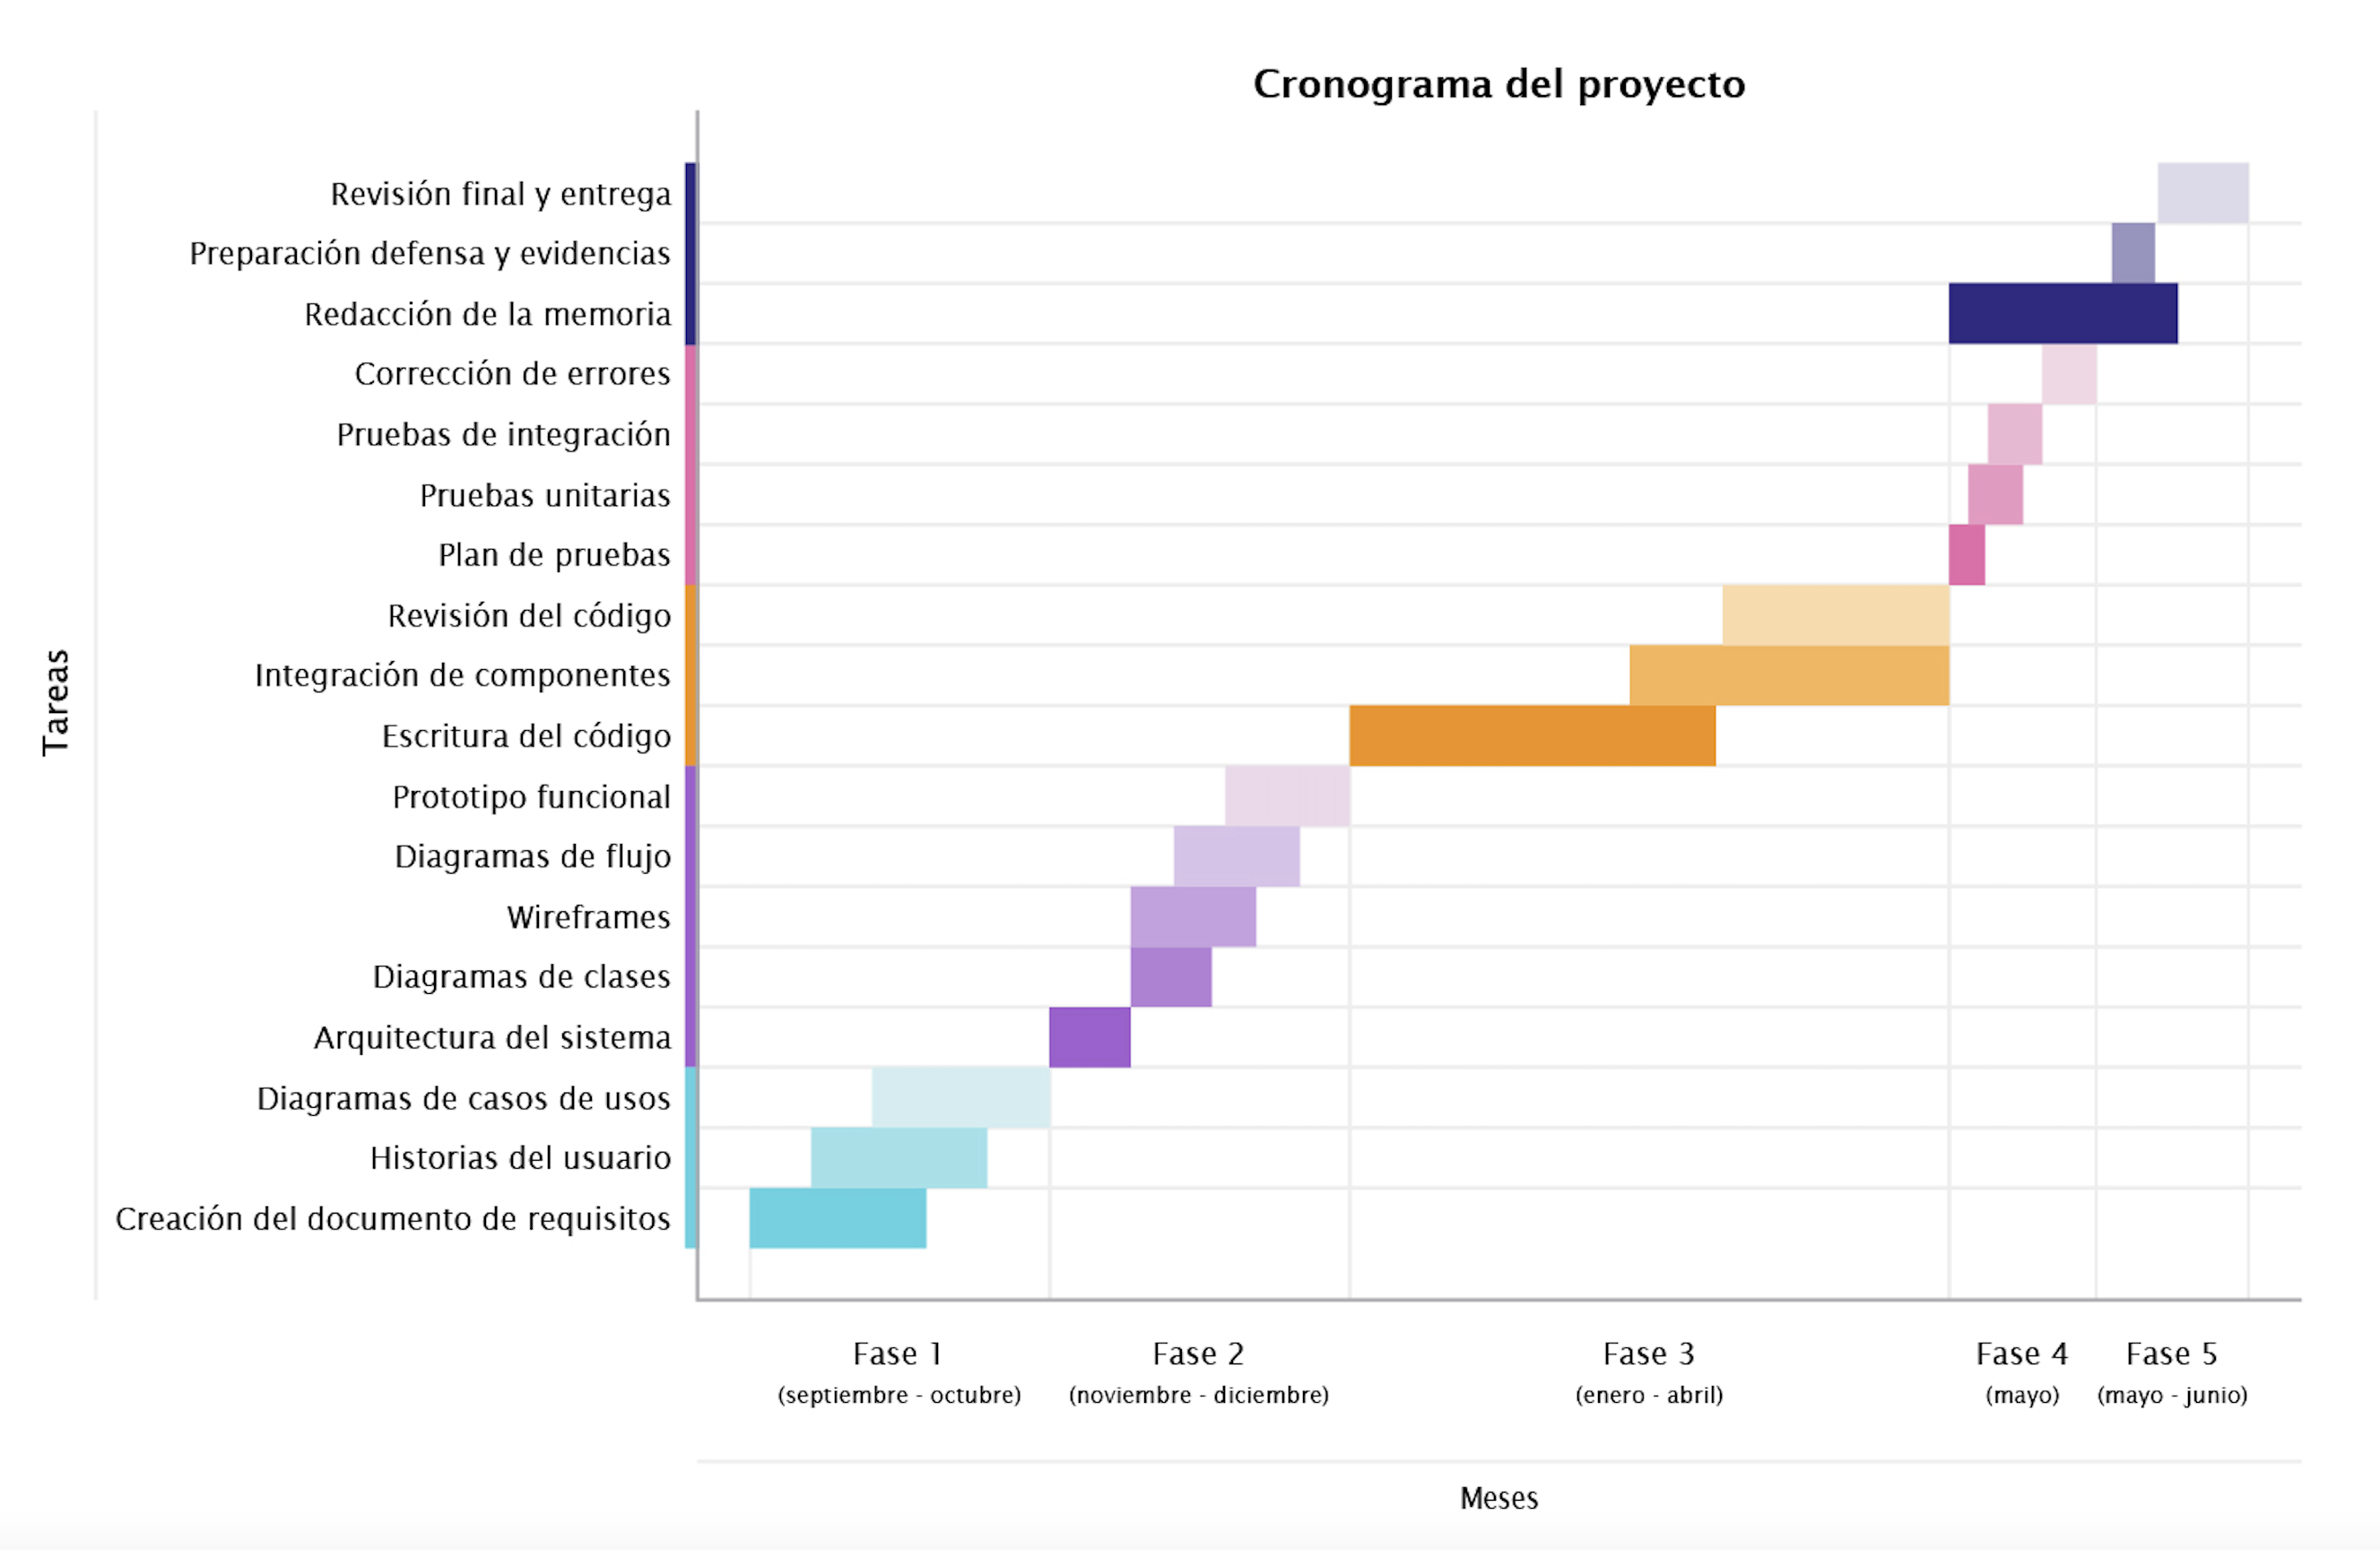
\includegraphics[width=1\textwidth]{Cronograma_TFG.png}
    \caption{Cronograma visual del proyecto, agrupado por fases y tareas.}
    \label{fig:cronograma}
\end{figure}


\subsection{Planificación de recursos}

\textbf{Recursos humanos:}
\begin{itemize}
    \item Alumna: Carlota de la Vega Soriano, encargada de todo el ciclo de vida del desarrollo.
    \item Tutor académico: Jesús Chamorro Martínez, apoyo en la supervisión y validación del enfoque técnico y científico.
\end{itemize}

\textbf{Recursos técnicos:}
\begin{itemize}
    \item Ordenador personal (MacBook Pro 2019, CPU sin GPU dedicada).
    \item Plataformas de computación en la nube: Kaggle (30h/semana con GPU gratuita) y Google Colab Pro (100 unidades informáticas).
    \item Librerías y frameworks: \texttt{PyTorch}, \texttt{TensorFlow}, \texttt{Keras}, \texttt{diffusers}, \texttt{transformers}, \texttt{Matplotlib}, entre otras.
    \item Datasets utilizados: MNIST, CIFAR-10/100, COCO, Stanford Dogs.
\end{itemize}

\textbf{Recursos software adicionales:}
\begin{itemize}
    \item Google Drive para gestión de datasets y modelos.
    \item Jupyter Notebooks y entornos virtuales gestionados con \texttt{Poetry}.
    \item Repositorios oficiales de Hugging Face y GitHub para pruebas con modelos preentrenados.
\end{itemize}

\subsection{Planificación económica}

El presupuesto inicial estimado fue el siguiente:

\begin{table}[ht]
    \centering
    \renewcommand{\arraystretch}{1.5}
    \begin{tabular}{p{5cm} >{\centering\arraybackslash}p{3cm} >{\centering\arraybackslash}p{3cm} >{\centering\arraybackslash}p{3cm} >{\centering\arraybackslash}p{3cm}}
        \rowcolor{gray!30}
        \textbf{Gastos elegibles} & \textbf{Unidades} & \textbf{Coste por unidad} & \textbf{Importe solicitado} \\
        \rowcolor{gray!20}
        GASTOS DE PERSONAL & & & \\
        \addlinespace
        Total gastos de contratación de personal & 1 & 10.71€/h & 4284€\\
        \rowcolor{gray!20}
        GASTOS DE EJECUCIÓN & & & \\
        Ordenador (Precio: 2462€) & 1 & 118.37€ & 118.37€ \\
        \addlinespace
        Servidor para ejecución & 1 & 0.899€/h & 359.60€ \\
         \addlinespace
        \rowcolor{gray!20}
        Costes indirectos (10\% presupuesto total) & & & 476.20€ \\
        \rowcolor{gray!30}
        \textbf{Total incentivo solicitado} &  & & \textbf{5238.17€} \\
    \end{tabular}
    \caption{Presupuesto del proyecto}
    \label{tab:presupuesto}
\end{table}


\subsection{Ajustes realizados sobre la planificación inicial}

Durante el desarrollo del trabajo, se han producido diversos ajustes sobre la planificación inicial, que reflejan tanto dificultades técnicas como decisiones informadas para optimizar el rendimiento:

\begin{itemize}
    \item \textbf{Cambio de framework}: aunque inicialmente se planteó el uso de \texttt{TensorFlow}, se decidió migrar a \texttt{PyTorch} para trabajar con AttnGAN y Stable Diffusion de forma más estable y con mejor soporte en la comunidad investigadora.
    
    \item \textbf{Uso de modelos preentrenados}: debido a las limitaciones computacionales, especialmente en Google Colab, se optó en parte por utilizar versiones preentrenadas de modelos como AttnGAN y Stable Diffusion (v1.5 y XL), evaluando su rendimiento sin necesidad de entrenamiento completo desde cero.
    
    \item \textbf{División del dataset COCO}: se decidió trabajar con subconjuntos seleccionados aleatoriamente debido a restricciones de memoria en entornos gratuitos.
    
    \item \textbf{Cambio de estrategia de representación textual}: se probaron distintas técnicas (One-Hot, Word2Vec), pero se optó finalmente por utilizar las descripciones originales del dataset COCO preprocesadas, mejorando así la eficiencia y preservando el contenido semántico.
    
    \item \textbf{Evaluación iterativa}: se optó por entrenamientos cortos con cambios progresivos en hiperparámetros, en lugar de una única sesión extensa, para facilitar el análisis comparativo de resultados.
\end{itemize}

Estas adaptaciones han permitido mantener la viabilidad del proyecto sin comprometer sus objetivos, y han fomentado la toma de decisiones técnicas fundamentadas, muy valiosas en un entorno profesional real.
